% ============PREAMBLE SECTION==========================================
%+++++++++++++++++++++++++++++++++++++++++++++++++++++++++++++++++++++++
\documentclass[12pt]{article}
\usepackage{geometry}                % See geometry.pdf to learn the layout options. There are lots.
\geometry{letterpaper}                   % ... or a4paper or a5paper or ... 
%\geometry{landscape}                % Activate for for rotated page geometry
\usepackage[parfill]{parskip}    % Activate to begin paragraphs with an empty line rather than an indent
\usepackage{daves,fancyhdr,natbib,graphicx,dcolumn,amsmath,lastpage,url}
\usepackage{amsmath,amssymb,epstopdf,longtable}
\DeclareGraphicsRule{.tif}{png}{.png}{`convert #1 `dirname #1`/`basename #1 .tif`.png}
\pagestyle{fancy}
\lhead{Student Name: \_\_\_\_\_\_\_\_\_\_\_\_\_\_\_\_\_\_\_\_\_\_\_\_\_\_\_\_\_\_\_\_\_\_\_\_\_\_\_\_\_\_\_\_\_ }
\rhead{FALL 2015}
\lfoot{CE 3354 Engineering Hydrology }
\cfoot{EXAM 1}
\rfoot{Page \thepage\ of \pageref{LastPage}}
\renewcommand\headrulewidth{0pt}

% other
\usepackage{paralist}  % need to modify standard enumerate blocks
%=========Longtable environment
\usepackage{setspace}                % allow single and double space environment
\usepackage{longtable}                % allow table to span multiple pages
\usepackage{caption}                    % consistent caption package
\usepackage{url}					% Ubiquitious url formatting package
%===========

\DeclareGraphicsRule{.tif}{png}{.png}{`convert #1 `dirname #1`/`basename #1 .tif`.png}
%++++++++++++++++++++++++++++++++++++++++++++++++++++++++++++++++++++++++++
%============================================================================
\begin{document}

\begingroup
\begin{centering}
\textbf{CE 3354 Engineering Hydrology} \\
\textbf{Exam 1, Fall 2015}\\
\end{centering}
~\\
Students should write their name on all sheets of paper.  
Students are permitted to use Laptops, Tablets, and smart phones for \textbf{browsing} the internet to help answer questions.  Students are permitted to use their own notes and the textbook to help answer questions.
\endgroup
%%%%%%%%%%%%%%%%%%%%%%%%%%%%%%%%%%%%%%%%%%%%%%%%%%%%%%
\begin{enumerate}
%%%%%% MULTIPLE GUESS PORTION %%%%%%%%%%%%%%%%%%%%
\item Hydrology is
\begin{enumerate}[a)]
\item Study of the atmosphere, ocean, and surface waters
\item The study of the occurrence, distribution, and movement of water above, on, and below the surface of the earth
\item A study of the processes of evaporation, infiltration, and storage
\item The study of the relationship between rainfall and runoff
\end{enumerate}
\item The fundamental unit of hydrology is ?
\begin{enumerate}[a)]
\item The rainfall depth
\item The main channel length
\item The main channel slope
\item The watershed 
\end{enumerate}
\item What is the relationship between the Annual Exceedance Probability (AEP) and the Annual Recurrence Interval (ARI)?
\begin{enumerate}[a)]
\item	The ARI is the average number of years between years containing one or more events exceeding a prescribed magnitude
\item	The AEP and ARI are the multiplicative inverse of one another
\item	The AEP is a plot of probability and magnitude
\item	The ARI is a plot of probability and magnitude
\end{enumerate}

\item An annual recurrence interval of 100-years is equivalent to an AEP of what percent?
\begin{enumerate}[a)]
\item 1-percent.
\item 10-percent.
\item 50-percent.
\item 100-percent.
\end{enumerate}
\item What is a flood frequency curve?
\begin{enumerate}[a)]
\item A plot of the discharge magnitude and the Weibull plotting position
\item A plot of the frequency and discharge
\item A plot of estimated exceedance probability and discharge
\item A plot of discharge and time
\end{enumerate}
\item What is a plotting position?
\begin{enumerate}[a)]
\item Location in a chart of a data pair
\item The multiplicative inverse of relative frequency
\item An estimate of probability associated with an observation based on its position within a ranked sample set
\item An estimate of probability associated with an observation based on its magnitude relative to the arithmetic mean
\end{enumerate}
\item To what type of data series would we apply the Bulletin 17C procedure ?
\begin{enumerate}[a)]
\item Annual maximum rainfall
\item Hourly rainfall
\item Annual maximum discharge
\item Instantaneous discharge
\end{enumerate}
\item Rainfall behavior is expressed as a combination of 
\begin{enumerate}[a)]
\item depth and duration
\item intensity and probability or frequency
\item duration and probability or frequency
\item depth or intensity, duration, and probability or frequency
\end{enumerate}
\item Rainfall intensity is 
\begin{enumerate}[a)]
\item the ratio of accumulated depth to duration
\item instantaneous rainfall rate
\item slope of the depth duration curve at a duration of one hour
\item integral of the depth duration curve from 0 to 24 hours
\end{enumerate}

\newpage
%%%%%%%%%%%%%%%%%%%%%%%%%%%%%%%%%%%%%%%%%%%%%%%%%%%%
\item Figure \ref{fig:ddf-curve.jpg} is a depth-duration-frequency plot for precipitation.

\begin{figure}[h!] %  figure placement: here, top, bottom, or page
   \centering
   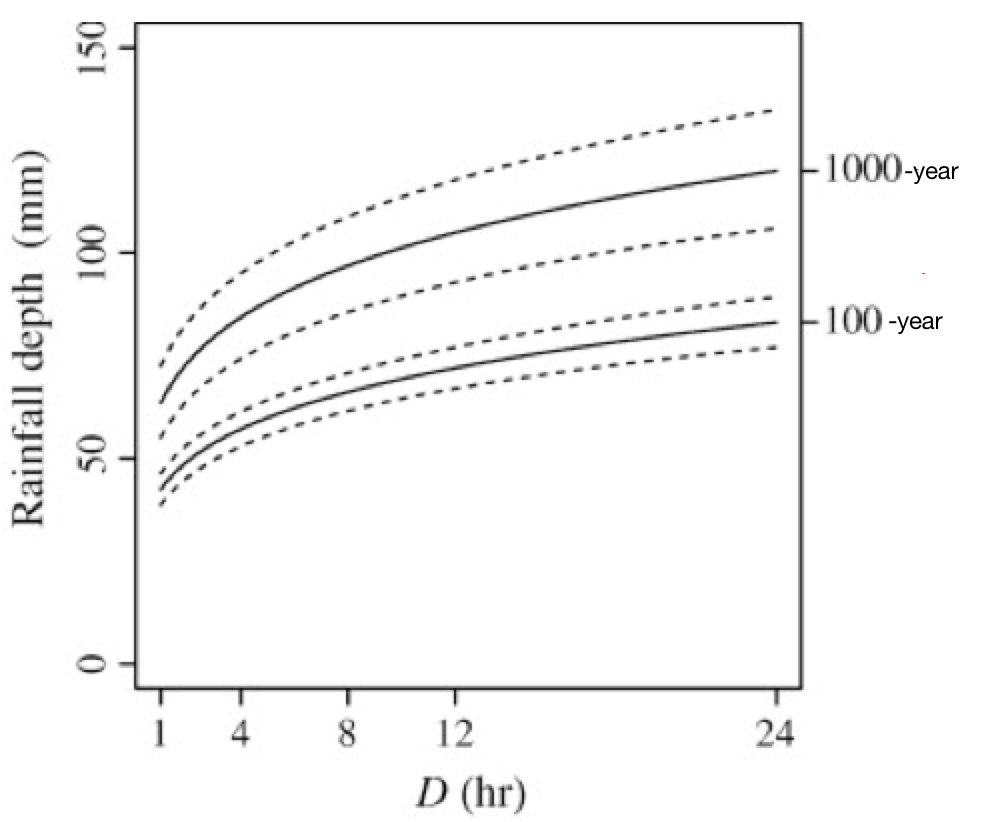
\includegraphics[width=6in]{ddf-curve.jpg} 
   \caption{Depth-duration-frequency curve}
   \label{fig:ddf-curve.jpg}
\end{figure}

The approximate depth, in millimeters, for a 4 hour, 100-yr (1\% chance) storm is 
\begin{enumerate}[a)]
\item 125 millimeters
\item 75 millimeters
\item 55 millimeters
\item 45 millimeters
\end{enumerate}
\clearpage



\begin{figure}[h!] %  figure placement: here, top, bottom, or page
   \centering
   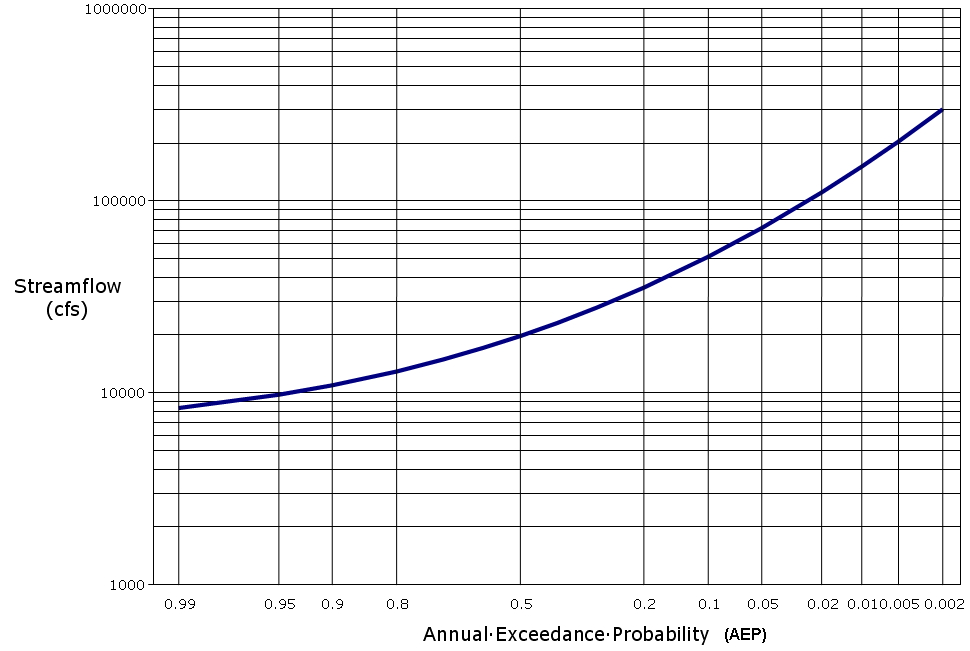
\includegraphics[width=6in]{flood-frequency-curve.jpg} 
   \caption{Flood frequency curve for a gaging station}
   \label{fig:flood-frequency-curve.jpg}
\end{figure}

\item Figure \ref{fig:flood-frequency-curve.jpg} is a flood frequency curve.   The probability of observing a discharge of magnitude of $50,000~CFS$ or more is
\begin{enumerate}[(a)]
\item $0.01$
\item $0.05$
\item $0.10$
\item $0.50$
\end{enumerate}

\item The median discharge from Figure \ref{fig:flood-frequency-curve.jpg} is
\begin{enumerate}[(a)]
\item $10,000~CFS$
\item $20,000~CFS$
\item $50,000~CFS$
\item $90,000~CFS$
\end{enumerate}

\clearpage

%%%%%%%%%%%%%%%%%%%%%%%%%% From ES1-P4 %%%%%%%%%%%%%%%%%%%%%%%%%%
\item The equation $k\frac{dQ}{dt} + Q(t) = I(t)$ is used to describe the response of streamflow to a constant rate of precipitation applied indefinitely on some watershed.  

Suppose that $Q(t)=0$ for $t=0$, the watershed characteristic time constant is $k=2~hrs$, and $I(t) =2$ for $t=[0,12)~hrs$ and then $I(t) =0$ for $t=[12,24]~hrs$. 

Determine:
\begin{enumerate}
\item The necessary equation(s) to predict the response $Q(t)$ over the 24-hour period.
\item Plot the values of $Q(t)$ over the 24-hour period (see next page for empty plot).
\end{enumerate}
\clearpage
~\newline
~\newline
~\newline
~\newline
~\newline
~\newline
~\newline
~\newline
~\newline
~\newline
~\newline
~\newline
~\newline
~\newline
\begin{figure}[h!] %  figure placement: here, top, bottom, or page
   \centering
   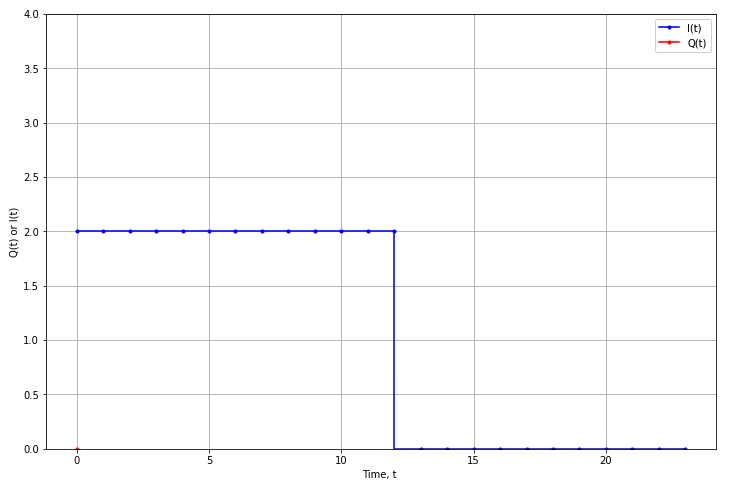
\includegraphics[width=6.0in]{HydrographPlot001.png} 
   \caption{Plot of Runoff for Watershed described by $k\frac{dQ}{dt} + Q(t) = I(t)$, where $I(t)$ is as shown (in blue)}
   \label{fig:topoMap.jpg}
\end{figure}
\clearpage
%%%%%%%%%%%%%%%%%%%%%%%%%%%%%%%%%%%%%%%%%%%%%%%%%%%%%%%%%%%%%%

%%%%%%%%%%%%%%%%%%%%% From ES-2 %%%%%%%%%%%%%%%%%%%%%%%%%%%%%%%
\item  Figure \ref{fig:topoMap.jpg} is a  topographic map of a small drainage basin.  The drawn contour interval is 20 feet.  Many of the contours are labeled.   A culvert structure is located on the Eastern portion of the basin, near the outlet shown on Figure \ref{fig:topoMap.jpg}.   The red line is a highway alignment, beneath which the culvert structure is placed.  Figure \ref{fig:Pan1.JPG} is a photograph of the culvert system that is comprised of 4-parallel , 4-foot diameter, 100-foot long culverts.  The lowest portion of the road near the culverts is at elevation 595 feet.  The culverts are laid on a dimensionless slope of $0.02$.

\begin{figure}[h!] %  figure placement: here, top, bottom, or page
   \centering
   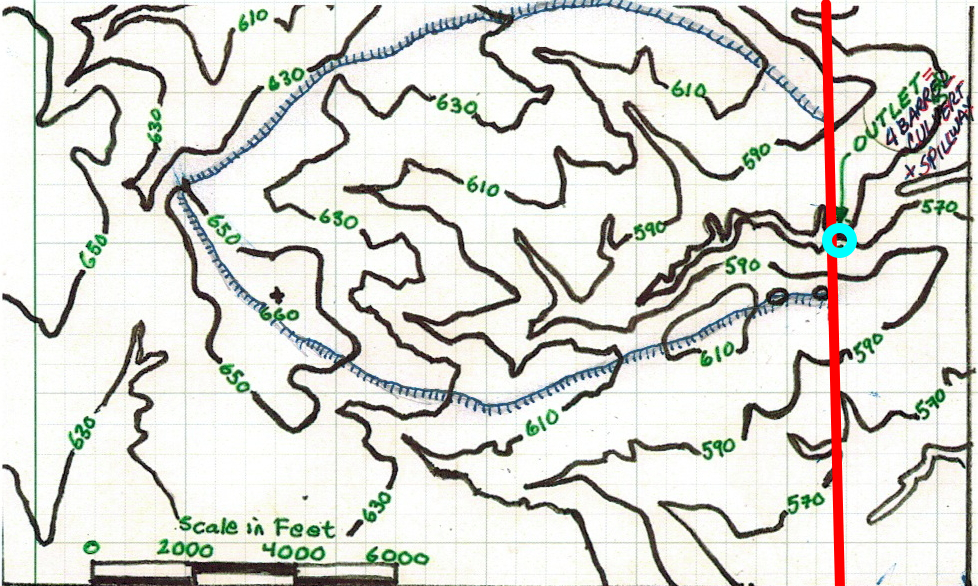
\includegraphics[width=6.5in]{topoMap.jpg} 
   \caption{Topographic Map of a portion of the Earth.  Elevations and linear distances are in $feet$. North (by convention) is up.}
   \label{fig:topoMap.jpg}
\end{figure}

\begin{figure}[h!] %  figure placement: here, top, bottom, or page
   \centering
   \includegraphics[width=6in]{Pan1.JPG} 
   \caption{Multiple-barrel outlet structure}
   \label{fig:Pan1.JPG}
\end{figure}
\clearpage

\begin{enumerate}[a)]
\item Estimate the drainage area in square feet of the drainage basin.   The boundary is already drawn on the map.
~\newline
~\newline
~\newline
~\newline
\item Convert the drainage area from square feet into acres.   
~\newline
~\newline
~\newline
~\newline
\item Convert the drainage area from acres into square miles.   
~\newline
~\newline
~\newline
~\newline
\item The water surface area when the culvert system (like a dam, with 4 holes in the wall) impounds water to a water surface elevation of $565~feet$ is essentially zero.  Complete the elevation (side) view sketch of the road embankment and culvert system in Figure \ref{fig:CulvertSystemElevation} by indicating the elevations on the sketch of the roadway crest, the culvert inlet elevation (also the upstream base of the embankment), and culvert outlet elevation.
\begin{figure}[h!] %  figure placement: here, top, bottom, or page
   \centering
   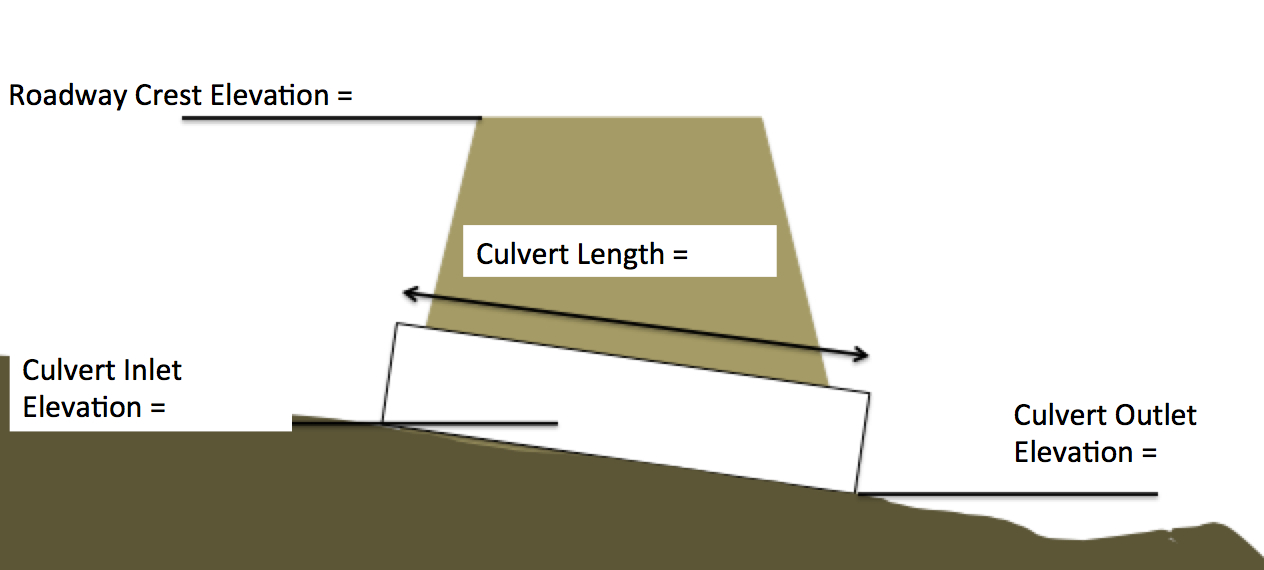
\includegraphics[height=2.6in]{CulvertSystemElevation.jpg} 
   \caption{Culvert system elevation view sketch}
   \label{fig:CulvertSystemElevation}
\end{figure}
\clearpage

\item Estimate the water surface area (area of the pool on the upstream side of the road embankment) when the embankment impounds water to a water surface elevation of $570~feet$.  Describe how you made the estimate.
~\newline
~\newline
~\newline
~\newline
~\newline
~\newline
~\newline
~\newline
~\newline
~\newline
\item Estimate the water surface area when the embankment impounds water to a water surface elevation of $580~feet$.  Describe how you made the estimate.
~\newline
~\newline
~\newline
~\newline
~\newline
~\newline
~\newline
~\newline
~\newline
~\newline
\item Estimate the water surface area when the embankment impounds water to a water surface elevation of $590~feet$.  Describe how you made the estimate.
~\newline
~\newline
~\newline
~\newline
~\newline
~\newline
~\newline
~\newline
~\newline
~\newline
\end{enumerate}
\clearpage

\item Figure~\ref{fig:RARO-DATA.pdf} is a tabulation of an observed storm and runoff for the drainage area depicted by the map in Figure~\ref{fig:topoMap.jpg}.  The runoff was measured before the installation of the roadway, at the location indicated by the blue circle on the map.


\begin{figure}[h!] %  figure placement: here, top, bottom, or page
   \centering
   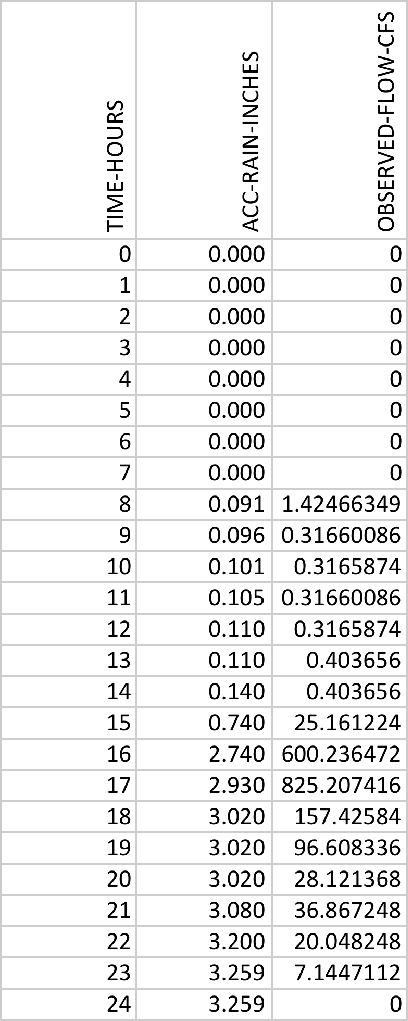
\includegraphics[width=2.5in]{RARO-DATA.pdf} 
   \caption{Cumulative rainfall for a 24-hour period on watershed determined for Figure \ref{fig:topoMap.jpg}}
   \label{fig:RARO-DATA.pdf}
\end{figure}
\clearpage
\begin{enumerate}[a)]
\item  Estimate the total \textbf{volume} of runoff in cubic feet from the storm.  Describe how you made your estimate.
~\newline
~\newline
~\newline
~\newline
~\newline
~\newline
~\newline
~\newline
\item Convert the estimate of runoff volume from cubic feet into watershed inches.
~\newline
~\newline
~\newline
~\newline
~\newline
~\newline
~\newline
\item How long (in hours) from the beginning of rainfall until the peak discharge occurs?
~\newline
~\newline
~\newline
~\newline
~\newline
\item What is the fraction of rainfall that becomes runoff?
\end{enumerate}
\clearpage

\end{enumerate}
\end{document}
%%%%%%%%%%%%%%%%%%%%%%%%%%%%%%%%%%%%%%%%%%%%%%%%%%%%%%%%%%%%%%%%%%%%%%%%
%%%%%%%%%%%%%%%%%%%%%%%%%%%%%%%%%%%%%%%%%%%%%%%%%%%%%%%%%%%%%%%%%%%%%%%%
\item How can one calculate the Annual Exceedance Probability (AEP) from the Annual Return Interval (ARI)?
\begin{enumerate}[a)]
\item	Cannot
\item	$AEP = \frac{1~yr}{ARI}$
\item	$ARI = \frac{1~yr}{AEP}$
\item	$ARI = \frac{Rank_i}{N+1}$
\end{enumerate}

%\item In the rational equation, $Q = CIA$, 
%\begin{enumerate}[a)]
%\item the intensity, $I$, is the ratio of depth to the time of concentration
%\item the intensity, $I$, is the ratio of depth to watershed area
%\item the intensity, $I$, is the ratio of depth to watershed discharge
%\item the intensity, $I$, is the ratio of depth to watershed impervious cover
%\end{enumerate}
%\item Regional analysis is used to
%\begin{enumerate}[a)]
%\item delineate watersheds
%\item relate discharge to drainage area
%\item construct regression equations from historical data on many streams within a region
%\item establish a typical functional drainage area
%\end{enumerate}

\item  The watershed in Figure \ref{fig:topoMap.jpg} is located in Briscoe County, Texas. Figure \ref{fig:countymap.pdf} is a map of
counties in Texas. Figures  \ref{fig:DDF-Atlas-5yr} and \ref{fig:DDF-Atlas-10yr} are excerpts from the Texas DDF Atlas.
\begin{enumerate}[a)]
\item Circle Briscoe county on Figure \ref{fig:countymap.pdf}.
\item Circle Briscoe county on Figure \ref{fig:DDF-Atlas-5yr}.
\item Circle Briscoe county on Figure \ref{fig:DDF-Atlas-10yr}.
\item Write the formula that converts the Annual Exceedence Probability (AEP) into an Annual Recurrence Interval (ARI).
~\newline
~\newline
~\newline
~\newline
~\newline
~\newline
~\newline
\item Estimate the precipitation depth in Brown county for a 2 hour storm with an Annual Exceedence Probability (AEP) of 0.2 (20 \%).
~\newline
~\newline
~\newline
~\newline
~\newline
~\newline
~\newline
\item Estimate the average rainfall intensity in Brown county for a 2 hour storm with an Annual Exceedence Probability (AEP) of 0.1 (10 \%).
~\newline
~\newline
~\newline
~\newline
~\newline
~\newline
~\newline
\end{enumerate}

\begin{figure}[h!] %  figure placement: here, top, bottom, or page
   \centering
   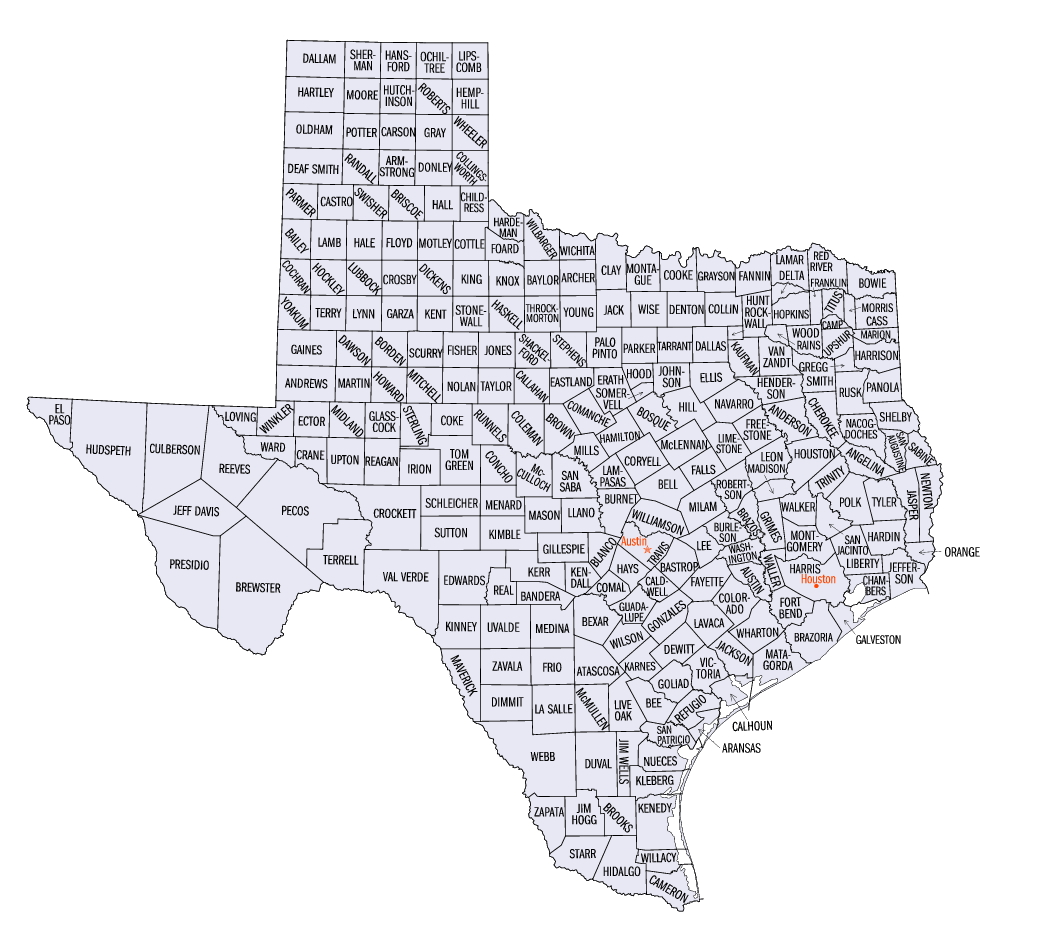
\includegraphics[width=6in]{countymap.jpg} 
   \caption{Cumulative rainfall for a 24-hour period on watershed determined for Figure \ref{fig:topoMap.jpg}}
   \label{fig:countymap.pdf}
\end{figure}

\begin{figure}[h!] %  figure placement: here, top, bottom, or page
   \centering
   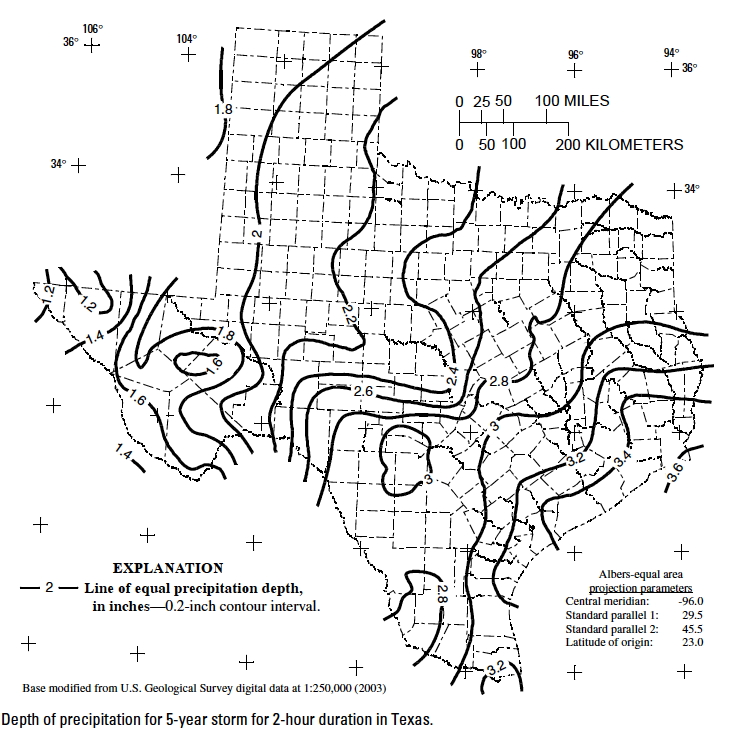
\includegraphics[width=6in]{DDF-Atlas-5yr.jpg} 
   \caption{Cumulative rainfall for a 24-hour period on watershed determined for Figure \ref{fig:topoMap.jpg}}
   \label{fig:DDF-Atlas-5yr}
\end{figure}

\begin{figure}[h!] %  figure placement: here, top, bottom, or page
   \centering
   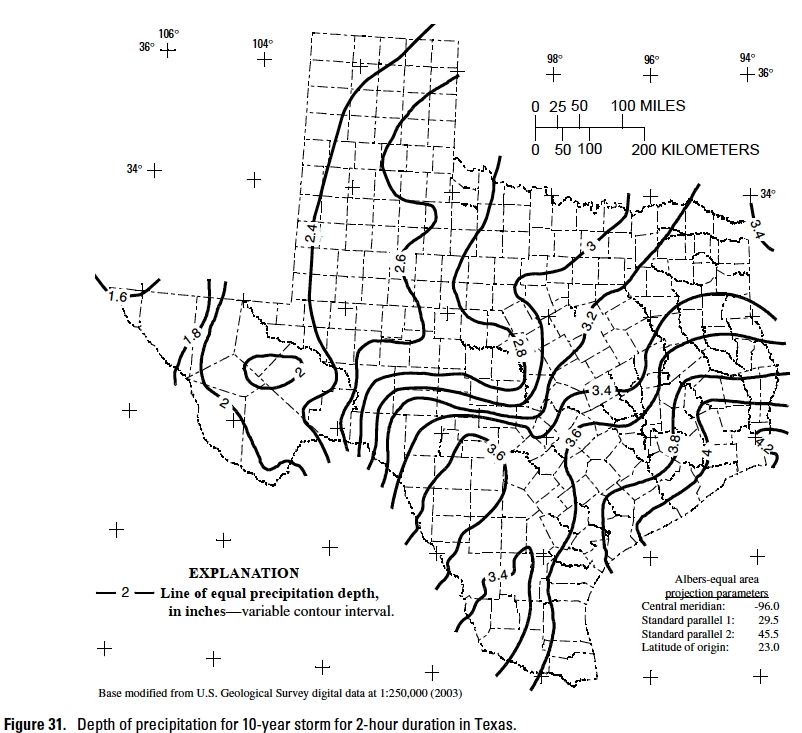
\includegraphics[width=6in]{DDF-Atlas-10yr.jpg} 
   \caption{Cumulative rainfall for a 24-hour period on watershed determined for Figure \ref{fig:topoMap.jpg}}
   \label{fig:DDF-Atlas-10yr}
\end{figure}

%
%
%
%
%
%
%
%
%~\\
